\documentclass{article}

\usepackage{postprocess/context/arxiv}

\usepackage[utf8]{inputenc} % allow utf-8 input
\usepackage{amsmath}
\usepackage[T1]{fontenc}    % use 8-bit T1 fonts
\usepackage{hyperref}       % hyperlinks
\usepackage{url}            % simple URL typesetting
\usepackage{booktabs}       % professional-quality tables
\usepackage{amsfonts}       % blackboard math symbols
\usepackage{nicefrac}       % compact symbols for 1/2, etc.
\usepackage{microtype}      % microtypography
\usepackage{graphicx}
\usepackage{natbib}
\usepackage{doi}
\usepackage{float}
\usepackage{subcaption}
\usepackage{wrapfig}

\title{Causal Discovery Report on Abalone}

\author{ \href{https://orcid.org/0000-0000-0000-0000}{
\includegraphics[scale=0.06]{postprocess/context/orcid.pdf}\hspace{1mm}\textbf{Causal Copilot}}}

\renewcommand{\headeright}{Technical Report}
\renewcommand{\undertitle}{Technical Report}

\hypersetup{
pdftitle={Causal Discovery Report on Abalone},
pdfauthor={Causal Copilot},
pdfkeywords={Causal Discovery, Large Language Model, PC, Abalone},
}

\begin{document}
\maketitle

\begin{abstract}
This report investigates the causal relationships present in a dataset containing anatomical and physical characteristics of abalones, a marine mollusk of notable economic and ecological importance. The analysis employs causal discovery methodologies, including the PC, Greedy Equivalence Search (GES), and DirectLiNGAM algorithms. Data preprocessing, algorithm selection, and hyperparameter tuning were guided by a large language model to enhance the robustness of the findings. The results demonstrate that age significantly influences various biological metrics, such as diameter and viscera weight, while length and height play critical roles in shaping overall biomass. Moreover, reliability analysis indicates substantial confidence in key causal relationships, though some statistically weak edges, aligned with biological context, require further investigation. This study contributes to a deeper understanding of abalone biology, with implications for sustainable fishing practices and conservation strategies.
\end{abstract}

\keywords{Causal Discovery, Large Language Model, PC, Abalone}

\raggedbottom
\section{Introduction}
This report aims to explore the causal relationships within a dataset that encompasses the anatomical and physical characteristics of abalones, a type of marine mollusk known for its economic and ecological significance. The dataset includes variables such as age, length, diameter, height, shell weight, whole weight, shucked weight, and viscera weight, all of which are interrelated and essential for assessing the growth and health of abalones. Analyzing these components can provide valuable insights into the growth patterns of abalones, influenced by factors such as environmental conditions and biological processes. By employing causal discovery methods, this study seeks to unravel the intricate dynamics among these variables, thereby contributing to a better understanding of abalone biology and informing sustainable fishing practices and conservation efforts.

\section{Background Knowledge}
\subsection{Detailed Explanation about the Variables}
\begin{itemize}
\item \textbf{Age}: Represents the age of the abalone, typically measured in years. It is derived from the number of rings on the shell. Understanding the age of abalones is vital for assessing growth patterns and reproductive status.
\item \textbf{Length}: The measurement of the abalone's length, usually in millimeters. This dimension is crucial as it may correlate with the age and overall health of the abalone. Length is often associated with the growth rate and can influence the market value of the abalone.
\item \textbf{Shell weight}: The weight of the shell itself, also in grams. The shell weight can influence the overall weight of the abalone and may vary with age and size. It is an essential characteristic for determining quality, especially in the seafood industry.
\item \textbf{Diameter}: The measurement of the abalone's shell diameter, measured in millimeters. This dimension complements the length measurement and helps in assessing the abalone's growth. Diameter measurements are useful for comparing growth rates among different populations or environments.
\item \textbf{Height}: The height of the abalone, measured in millimeters. This variable adds an additional dimension to the size profile of the abalone and aids in understanding its overall form and biomass.
\item \textbf{Whole weight}: The total weight of the abalone in grams, including the shell and all soft body parts. This is an important variable for assessing the overall biomass of the organism and is critical for commercial valuation.
\item \textbf{Shucked weight}: The weight of the abalone's meat after the shell has been removed, which is a relevant measure for commercial purposes, particularly in the seafood industry. This measurement is often used to calculate yield and profitability.
\item \textbf{Viscera weight}: The weight of the internal organs (guts) of the abalone, also measured in grams. This variable may provide insights into the health and reproductive status of the abalone, as visceral development can change with age and environmental conditions.
\end{itemize}

Together, these variables provide a comprehensive understanding of the physical characteristics and potential growth dynamics of abalones, which are crucial for both ecological study and commercial exploitation.

\subsection{Possible Causal Relations among these Variables}

\begin{minipage}[t]{0.7\linewidth}
\begin{itemize}
    \item \textbf{Age $\rightarrow$ Length}: As abalones age, they typically grow in size, leading to an increase in length.
    \item \textbf{Age $\rightarrow$ Diameter}: Older abalones tend to have larger diameters due to their overall growth patterns associated with age.
    \item \textbf{Age $\rightarrow$ Height}: The height measurement of abalones increases with age as they continue to grow larger over time.
    \item \textbf{Age $\rightarrow$ Shell weight}: With age, abalones develop heavier shells as they grow and build additional shell material.
    \item \textbf{Age $\rightarrow$ Whole weight}: The whole weight of an abalone increases with age due to overall growth in size and volume of its body.
    \item \textbf{Age $\rightarrow$ Shucked weight}: Older abalones generally yield more meat, resulting in a higher shucked weight.
    \item \textbf{Age $\rightarrow$ Viscera weight}: The weight of the internal organs increases with age, as older abalones may develop larger and heavier internal structures.
    \item \textbf{Length $\rightarrow$ Whole weight}: As the length of the abalone increases, the total whole weight typically rises because longer abalones usually have more body mass.
    \item \textbf{Diameter $\rightarrow$ Whole weight}: A larger diameter indicates a more substantial body structure, which contributes to an increase in whole weight.
    \item \textbf{Height $\rightarrow$ Whole weight}: The height of an abalone contributes to its overall biomass, thus impacting the whole weight.
    \item \textbf{Shell weight $\rightarrow$ Whole weight}: The shell weight is a significant component of the total whole weight, as it adds to the overall mass of the abalone.
    \item \textbf{Shucked weight $\rightarrow$ Whole weight}: Shucked weight represents the meat portion of the abalone, which is part of the total whole weight.
    \item \textbf{Viscera weight $\rightarrow$ Whole weight}: The weight of the internal organs contributes to the overall weight of the abalone, hence affecting whole weight.
    \item \textbf{Length $\rightarrow$ Diameter}: Generally, an increase in length corresponds with an increase in diameter, as both are measures of the abalone's size.
    \item \textbf{Length $\rightarrow$ Height}: As the length increases, height tends to increase as well, reflecting the overall growth of the abalone.
    \item \textbf{Diameter $\rightarrow$ Height}: A larger shell diameter is often associated with an increase in height, as both dimensions provide a fuller representation of the abalone's physical growth.
    \item \textbf{Shell weight $\rightarrow$ Shucked weight}: The strength and integrity of the shell may correlate with the amount of meat, impacting the shucked weight.
    \item \textbf{Viscera weight $\rightarrow$ Shucked weight}: The weight of the internal organs may have a relationship with the amount of meat produced, thus affecting the shucked weight.
\end{itemize}
\end{minipage}
\hspace{0.05\textwidth}
\begin{minipage}[t]{0.3\linewidth}
    \begin{figure}[H]
        \centering
        \resizebox{\linewidth}{!}{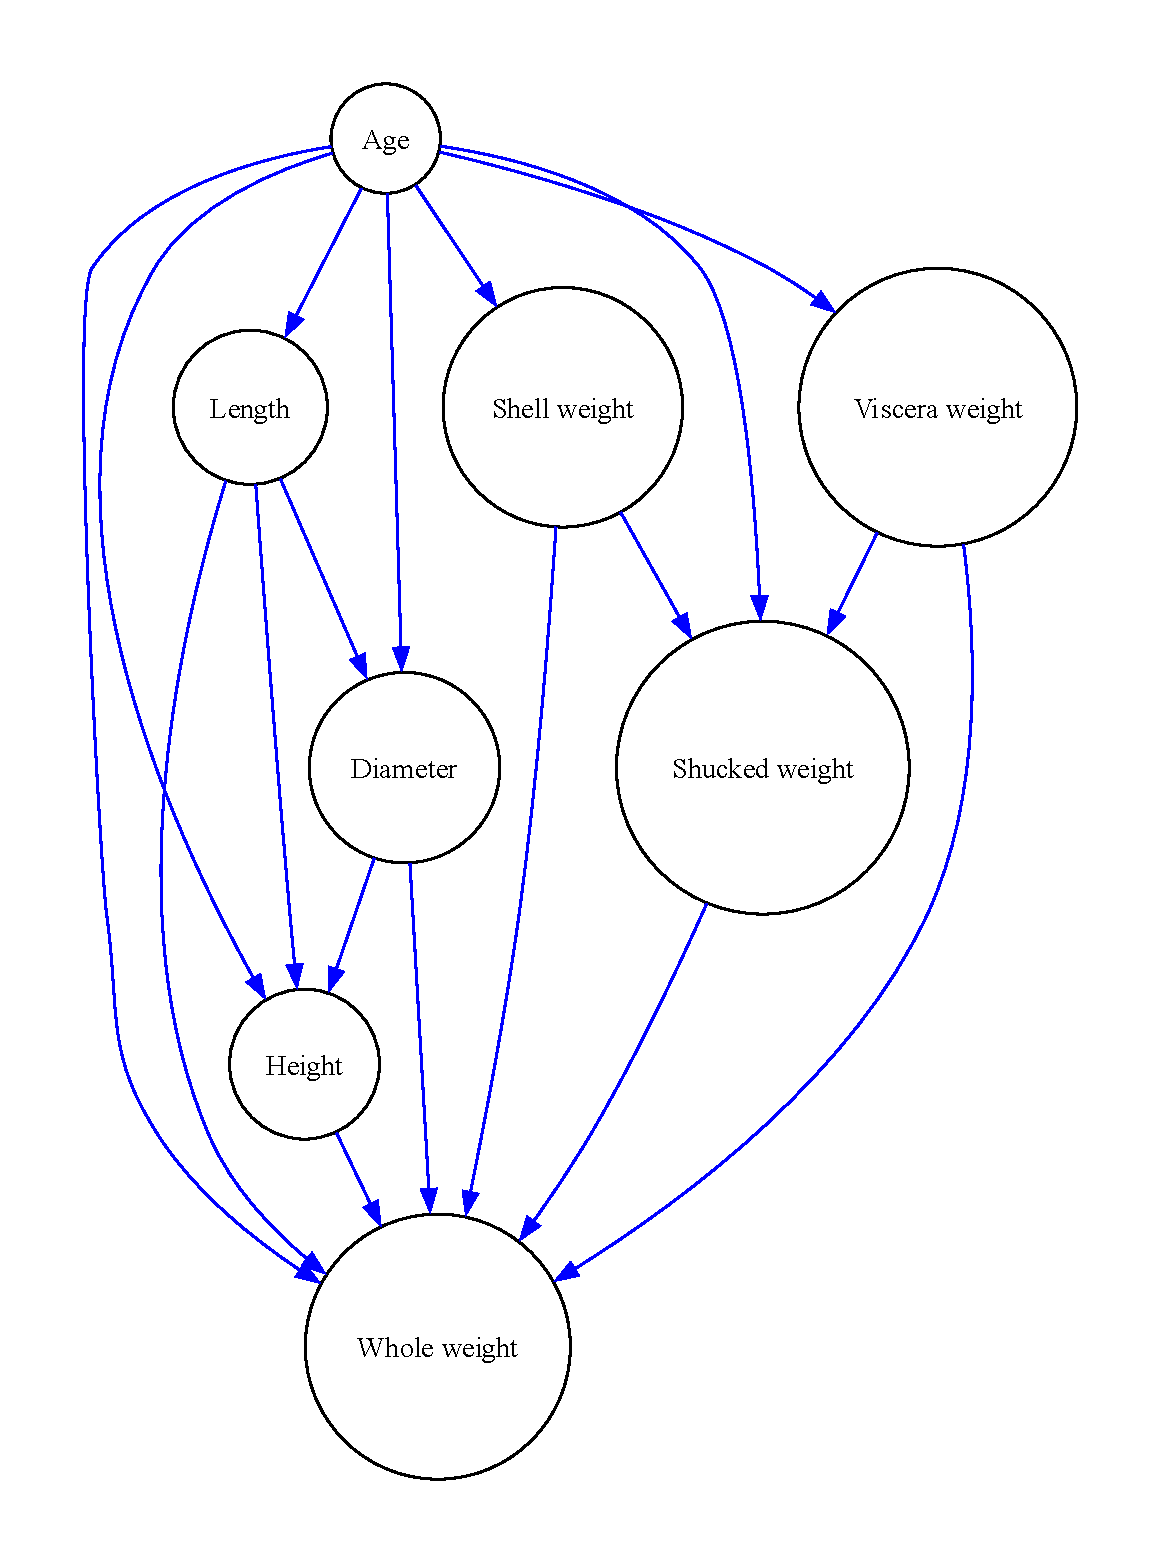
\includegraphics[height=0.4\textheight]{./demo_data/20241104_093143/Abalone/output_graph/potential_relation.pdf}}
        \caption{\label{fig:relation}Possible Causal Relation Graph}
    \end{figure}
\end{minipage}

\section{Dataset Descriptions and EDA}
The following is a preview of our original dataset.

\begin{table}[H]
    \centering
    \caption{Dataset Preview}
    \begin{tabular}{rrrrrrrr}
\toprule
 Age &  Length &  Shell weight &  Diameter &  Height &  Whole weight &  Shucked weight &  Viscera weight \\
\midrule
15.0 &   0.455 &         0.365 &     0.095 &  0.5140 &        0.2245 &          0.1010 &           0.150 \\
 7.0 &   0.350 &         0.265 &     0.090 &  0.2255 &        0.0995 &          0.0485 &           0.070 \\
 9.0 &   0.530 &         0.420 &     0.135 &  0.6770 &        0.2565 &          0.1415 &           0.210 \\
10.0 &   0.440 &         0.365 &     0.125 &  0.5160 &        0.2155 &          0.1140 &           0.155 \\
 7.0 &   0.330 &         0.255 &     0.080 &  0.2050 &        0.0895 &          0.0395 &           0.055 \\
\bottomrule
\end{tabular}
\end{table}

\subsection{Data Properties}
We employ several statistical methods to identify data properties.

The shape of the data, data types, and missing values are assessed directly from the dataframe.
Linearity is evaluated using Ramsey’s RESET test, followed by the Benjamini \& Yekutieli procedure for multiple test correction.
Gaussian noise is assessed through the Shapiro-Wilk test, also applying the Benjamini \& Yekutieli procedure for multiple test correction.
Time-Series and Heterogeneity are derived from user queries.

Properties of the dataset we analyzed are listed below.

\begin{table}[H]
    \centering
    \caption{Data Properties}

        \begin{tabular}{rrrrrrr}
            \toprule
            Shape ($n$ x $d$) & Data Type & Missing Value & Linearity & Gaussian Errors & Time-Series & Heterogeneity \\
            \midrule
            (4177, 8)   & Continuous & False & False & False & False & False \\
            \bottomrule
        \end{tabular}
        
\end{table}

\subsection{Distribution Analysis}
The following figure shows distributions of different variables. The orange dash line represents the mean, 
and the black line represents the median. Variables are categorized into three types according to their distribution characteristics.

\begin{figure}[H]
\centering
\includegraphics[width=\linewidth]{./demo_data/20241104_093143/Abalone/output_graph/eda_dist.jpg}
\caption{\label{fig:dist}Distribution Plots of Variables}
\end{figure}

\begin{itemize}
\item Slight left skew distributed variables: Length, Shell weight, Diameter, Whole weight
\item Slight right skew distributed variables: Age, Height, Shucked weight, Viscera weight
\item Symmetric distributed variables: None
\end{itemize}

\subsection{Correlation Analysis}

\begin{minipage}[t]{0.5\linewidth}
    In this analysis, we will categorize the correlation statistics of features in the dataset into three distinct categories: Strong correlations, Moderate correlations, and Weak correlations.

\begin{itemize}
\item Strong Correlated Variables: Shell weight and Length, Height and Whole weight, Viscera weight and Shell weight, Shucked weight and Height, Shucked weight and Shell weight, Viscera weight and Height, Viscera weight and Shucked weight, Shucked weight and Whole weight, Whole weight and Height
\item Moderate Correlated Variables: Length and Age, Shell weight and Age, Diameter and Age, Diameter and Length, Diameter and Shell weight, Height and Age, Height and Length, Height and Diameter, Whole weight and Diameter, Whole weight and Length, Shucked weight and Diameter, Viscera weight and Age
\item Weak Correlated Variables: Shucked weight and Age
\end{itemize}
\vfill
\end{minipage}
\hfill
\begin{minipage}[t]{0.5\linewidth}
    \begin{figure}[H]
        \centering
        \vspace{-1.5cm}
        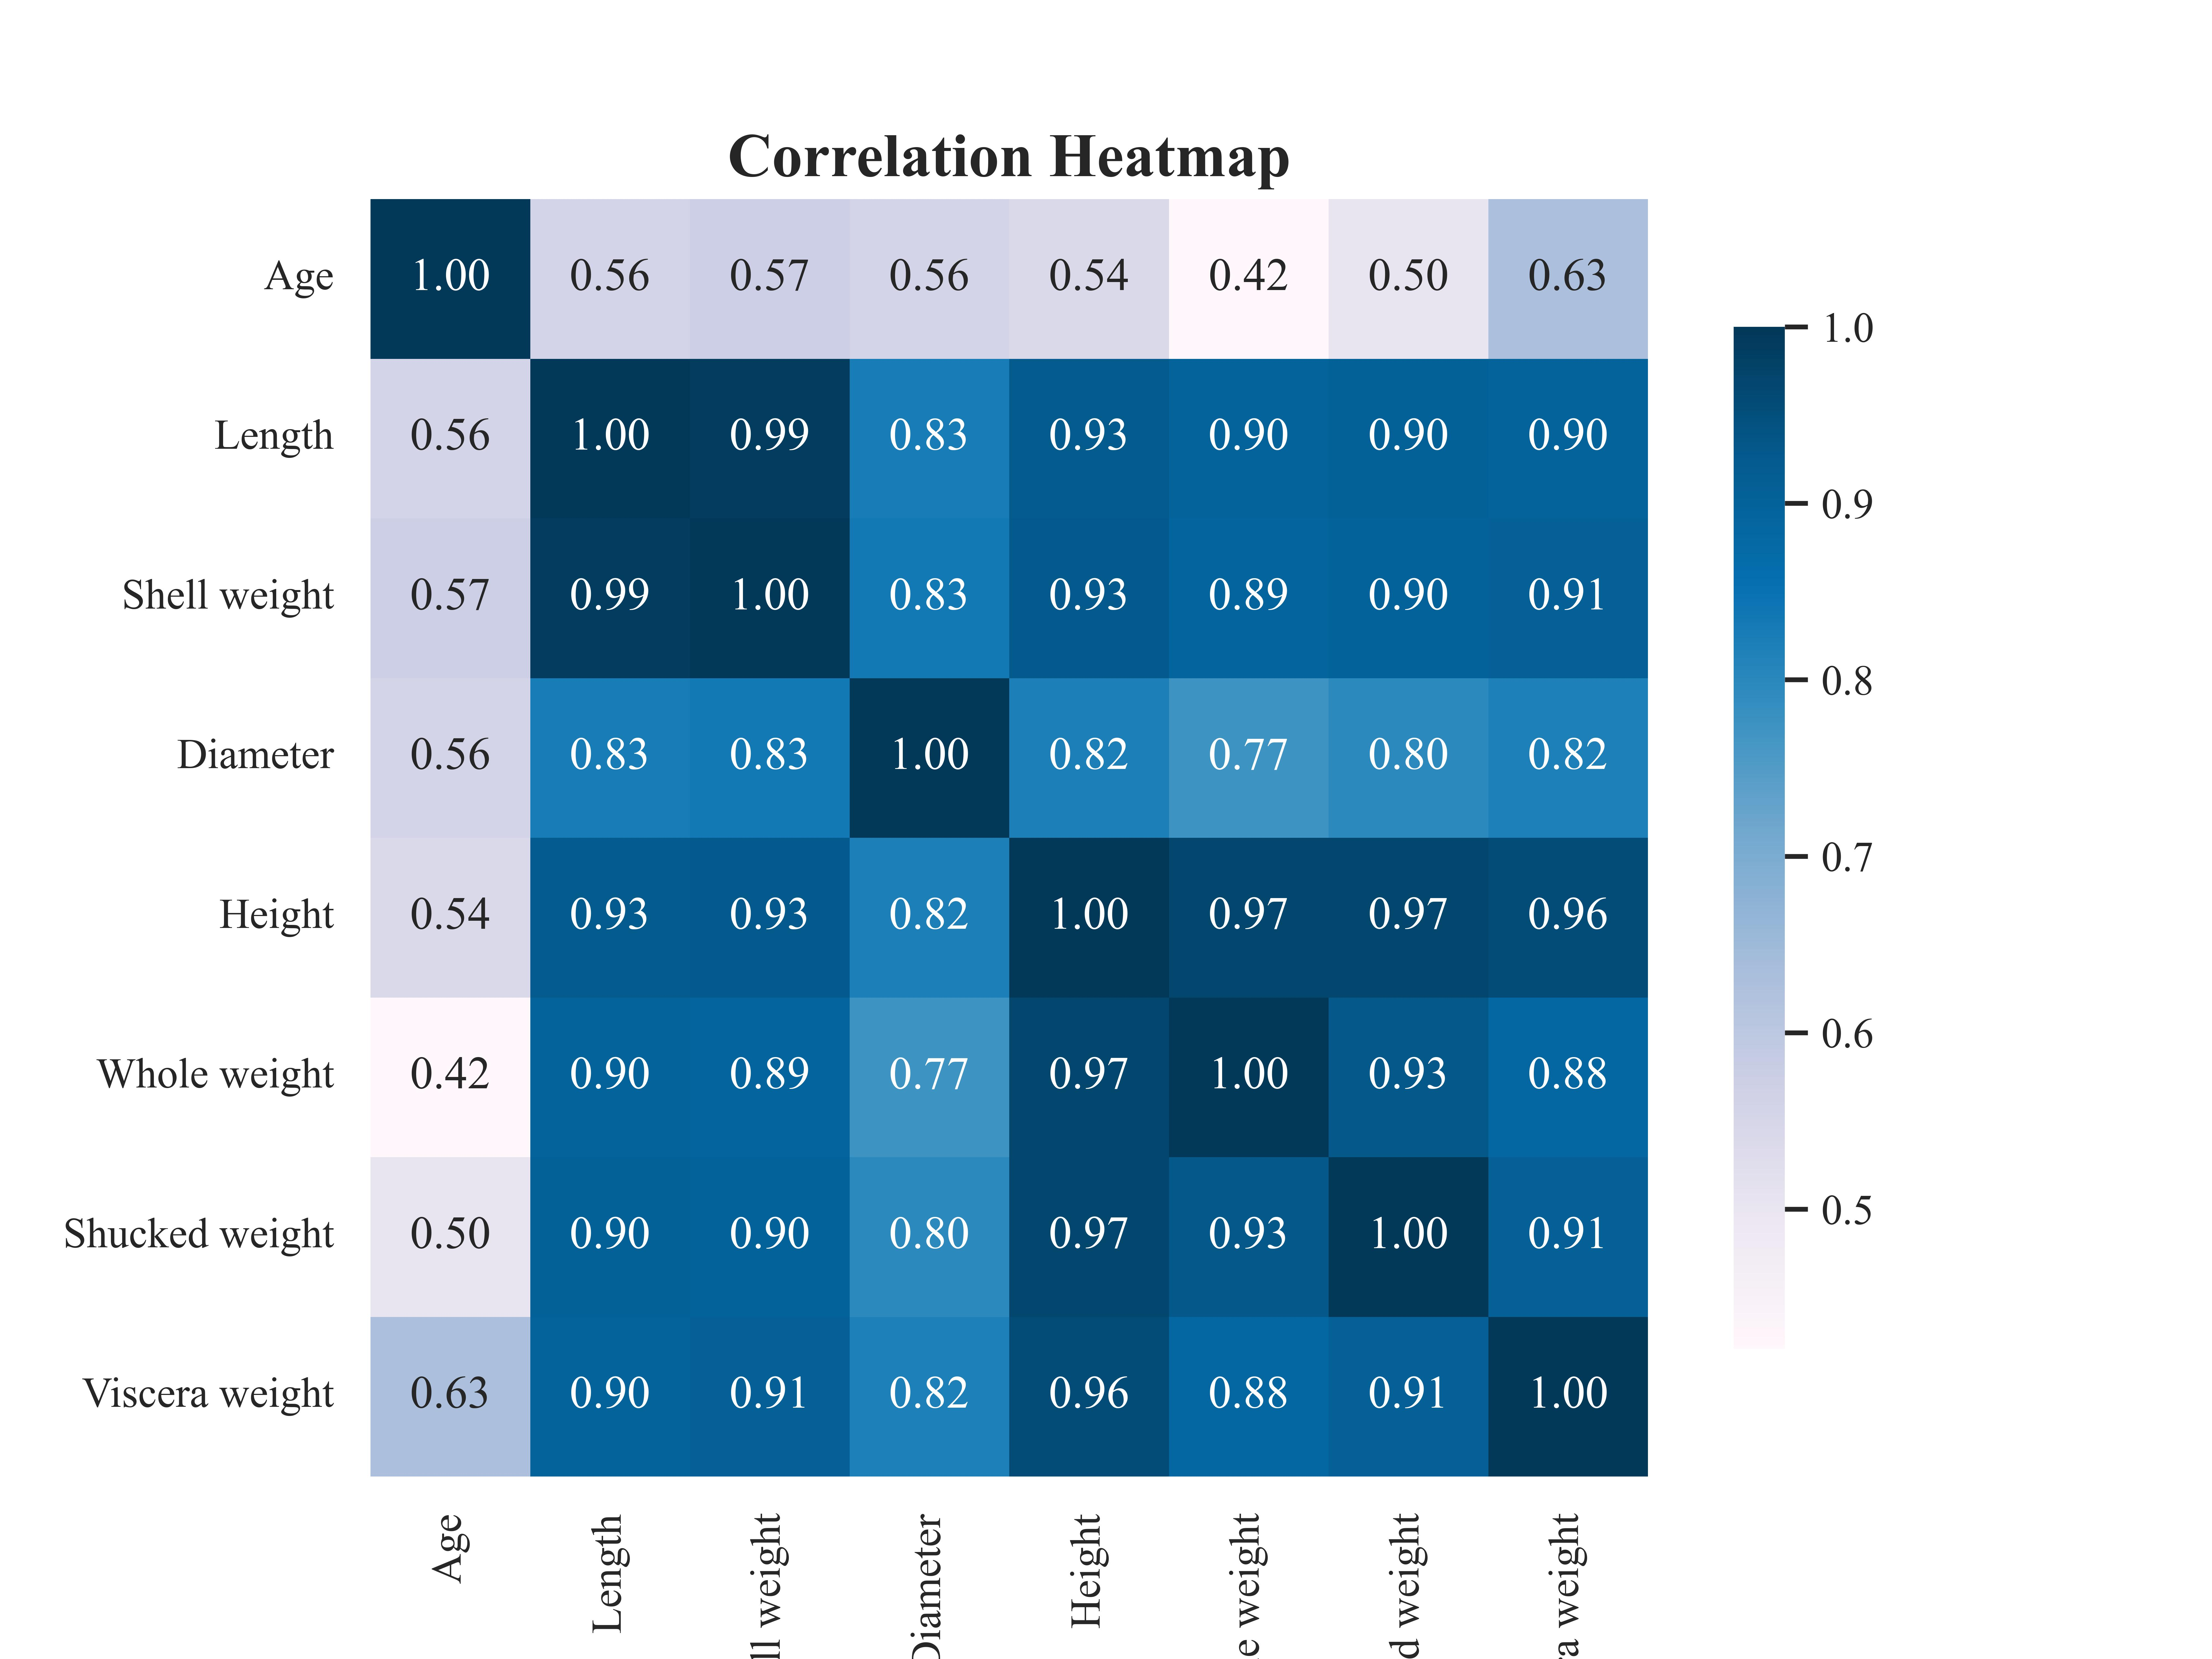
\includegraphics[width=\linewidth]{./demo_data/20241104_093143/Abalone/output_graph/eda_corr.jpg}
        \caption{\label{fig:corr}Correlation Heatmap of Variables}
    \end{figure}
\end{minipage}

\section{Discovery Procedure}

In this section, we provide a detailed description of the causal discovery process implemented by Causal Copilot. 
We also provide the chosen algorithms and hyperparameters, along with the justifications for these selections.

\subsection{Data Preprocessing}
In this initial step, we preprocessed the data and examined its statistical characteristics. 
This involved cleaning the data, handling missing values, and performing exploratory data analysis to understand distributions and relationships between variables.
                
\subsection{Algorithm Selection assisted with LLM}
Following data preprocessing, we employed a large language model (LLM) to assist in 
selecting appropriate algorithms for causal discovery based on the statistical characteristics of the dataset and relevant background knowledge. 
The top three chosen algorithms, listed in order of suitability, are as follows:   

\begin{itemize}
    \item \textbf{PC}:
    \begin{itemize}
        \item \textbf{Description}: The PC algorithm is a constraint-based method that learns the structure of a causal graph from data by testing conditional independencies between variables. It constructs a directed acyclic graph (DAG) representing the causal relationships.
        \item \textbf{Justification}: Given the large sample size of 4177 and the absence of missing values, the PC algorithm is suitable as it efficiently handles large datasets and all relevant variables are observed, allowing for the identification of a causal structure.
    \end{itemize}

    \item \textbf{GES}:
    \begin{itemize}
        \item \textbf{Description}: Greedy Equivalence Search (GES) is a score-based causal discovery algorithm that identifies the optimal causal structure by navigating the space of equivalence classes of Directed Acyclic Graphs (DAGs).
        \item \textbf{Justification}: GES is appropriate due to the non-linear relationships present in the dataset and the large sample size. It provides a flexible approach that can leverage both Gaussian and non-Gaussian distributions, making it suitable given the dataset’s statistical properties.
    \end{itemize}

    \item \textbf{DirectLiNGAM}:
    \begin{itemize}
        \item \textbf{Description}: DirectLiNGAM is an efficient approach to causal discovery assuming linear relationships with non-Gaussian noise, designed to directly estimate the causal order.
        \item \textbf{Justification}: DirectLiNGAM is suitable given the high sample size and the assumption of non-Gaussian error distribution. Although the dataset doesn't exhibit predominant linearity, it can still be explored using this method to uncover causal relationships efficiently.
    \end{itemize}
\end{itemize}
        
\subsection{Hyperparameter Values Proposal assisted with LLM}
Once the algorithms were selected, the LLM aided in proposing hyperparameters 
for the chosen algorithm, which are specified below:
        
\begin{itemize}
    \item \textbf{alpha}:
    \begin{itemize}
        \item \textbf{Value}: 0.05
        \item \textbf{Explanation}: Given the sample size of 4177 is between 500 and 10000, the default significance level of 0.05 is appropriate. This balances the need for error control while providing sufficient power to detect dependencies in the dataset.
    \end{itemize}

    \item \textbf{findep\_test}:
    \begin{itemize}
        \item \textbf{Value}: fisherz
        \item \textbf{Explanation}: Since the dataset contains continuous data, 'fisherz' is the most suitable choice for the independence test, despite the known limitations regarding linearity and Gaussian errors. It is the default for continuous data types.
    \end{itemize}

    \item \textbf{depth}:
    \begin{itemize}
        \item \textbf{Value}: -1
        \item \textbf{Explanation}: With 8 features in the dataset, using unlimited depth (-1) allows for full exploration of possible relationships without imposing unnecessary constraints. This enhances the accuracy of the causal discovery process.
    \end{itemize}
\end{itemize}

\subsection{Graph Tuning with Bootstrap and LLM Suggestion}
In the final step, we performed graph tuning with suggestions provided by the Bootstrap and LLM.
            
Firstly, we use the Bootstrap technique to get how much confidence we have on each edge in the initial graph.
If the confidence probability of a certain edge is greater than 95\% and it is not in the initial graph, we force it.
Otherwise, if the confidence probability is smaller than 5\% and it exists in the initial graph, we change it to the edge type with the highest probability.
            
After that, we utilize LLM to help us prune edges and determine the direction of undirected edges according to its knowledge repository.
In this step, LLM can use background knowledge to add some edges that are neglected by Statistical Methods.
Voting techniques are used to enhance the robustness of results given by LLM, and the results given by LLM should not change results given by Bootstrap.

By integrating insights from both of Bootstrap and LLM to refine the causal graph, we can achieve improvements in graph's accuracy and robustness.
            

\section{Results Summary}

\subsection{Initial Graph}

\begin{figure}[H]
    \centering
    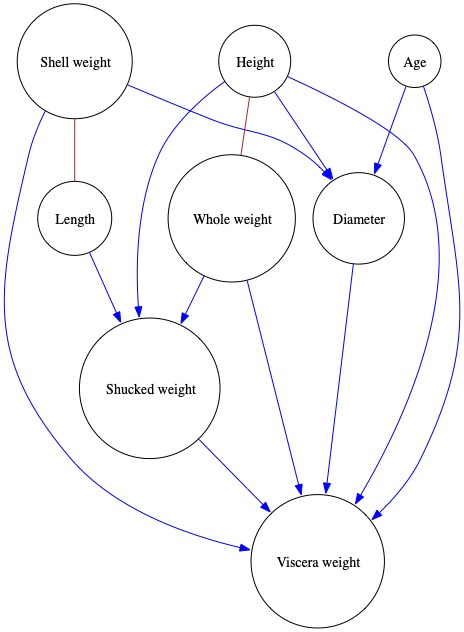
\includegraphics[width=\linewidth]{./demo_data/20241104_093143/Abalone/output_graph/initial_graph.pdf}
    \caption{Initial Graph}
\end{figure}

The above is the initial result graph produced by our algorithm.

The causal relationships among the variables indicate that Age plays a significant role in influencing various biological metrics, including Diameter and Viscera weight, highlighting the impact of maturation on these traits. Length appears to have a dual role, as it affects shell weight and shucked weight, which in turn have implications for both Diameter and Viscera weight, demonstrating the interconnectedness of physical dimensions with overall biomass. Height, as a crucial determinant, influences Diameter, Whole weight, Shucked weight, and Viscera weight, suggesting that as organisms grow taller, their overall size and internal mass increase proportionately. This cascade of effects reveals a complex interplay where one variable can have downstream impacts on others, ultimately shaping the overall physical characteristics and health of the organism. Thus, the relationships among these traits underscore the importance of age and size in the growth and development of organisms.

\subsection{Revised Graph}

\begin{minipage}[t]{0.6\linewidth}
    
By using the method mentioned in Section 4.4, we provide a revised graph pruned with Bootstrap and LLM suggestion.
Pruning results are as follows.
        
Bootstrap doesn't force or forbid any edges.
            
The following are forced results given by LLM:
            
\begin{itemize}
    \item \textbf{Age $\rightarrow$ Length}: Older abalones generally exhibit greater length due to biological growth patterns, as age is associated with increased size.
    \item \textbf{Age $\rightarrow$ Shell weight}: As abalones age, their shell becomes heavier, reflecting growth and development influenced by environmental factors.
    \item \textbf{Age $\rightarrow$ Height}: Increased age corresponds to greater height in abalones, contributing to overall size and health.
    \item \textbf{Age $\rightarrow$ Whole weight}: With age, the overall biomass of the abalone increases, leading to a heavier total weight as growth occurs in all body parts.
    \item \textbf{Age $\rightarrow$ Shucked weight}: Older abalones typically yield more meat due to natural growth over time, resulting in greater shucked weight.
    \item \textbf{Length $\rightarrow$ Diameter}: Length and diameter are interrelated dimensions of the abalone; as abalones grow longer, their diameter also tends to increase.
    \item \textbf{Length $\rightarrow$ Height}: These three dimensions (length, diameter, height) correlate with one another, as overall size affects each measurement.
    \item \textbf{Length $\rightarrow$ Whole weight}: Length contributes significantly to the total biomass of the abalone, as a larger length indicates a heavier mass.
    \item \textbf{Length $\rightarrow$ Viscera weight}: As abalones grow longer, the weight of their internal organs often increases, influenced by overall growth and health.
    \item \textbf{Shell weight $\rightarrow$ Height}: The weight of the shell affects the overall structure and size of the abalone, which includes its height.
    \item \textbf{Shell weight $\rightarrow$ Whole weight}: The shell weight is a significant component of the total weight, affecting the overall biomass of the abalone.
    \item \textbf{Shell weight $\rightarrow$ Shucked weight}: A heavier shell may correlate with greater meat content, leading to an increase in shucked weight when the shell is removed.
    \item \textbf{Diameter $\rightarrow$ Whole weight}: Diameter contributes to the size and mass of the abalone, directly affecting its total weight.
    \item \textbf{Diameter $\rightarrow$ Shucked weight}: Wider diameter may correlate with more meat production, thereby increasing the shucked weight as the abalone grows larger.
\end{itemize}
            
The following are directions of remaining undirected edges determined by the LLM:
\begin{itemize}
    \item \textbf{Length $\rightarrow$ Shell weight}: Length influences Shell weight since a larger abalone generally has a heavier shell due to its growth. As the length increases, the amount of material making up the shell also increases, resulting in increased shell weight.
    \item \textbf{Height $\rightarrow$ Whole weight}: Height impacts Whole weight because a taller abalone typically has more body mass and thus contributes to increased total weight. The height reflects physical dimensions that are related to the overall size and biomass of the organism.
\end{itemize}
            
This structured approach ensures a comprehensive and methodical analysis of the causal relationships within the dataset.
        
\vfill
\end{minipage}
\hfill
\begin{minipage}[t]{0.4\linewidth}
    \begin{figure}[H]
        \centering
        \vspace{-0.5cm}
        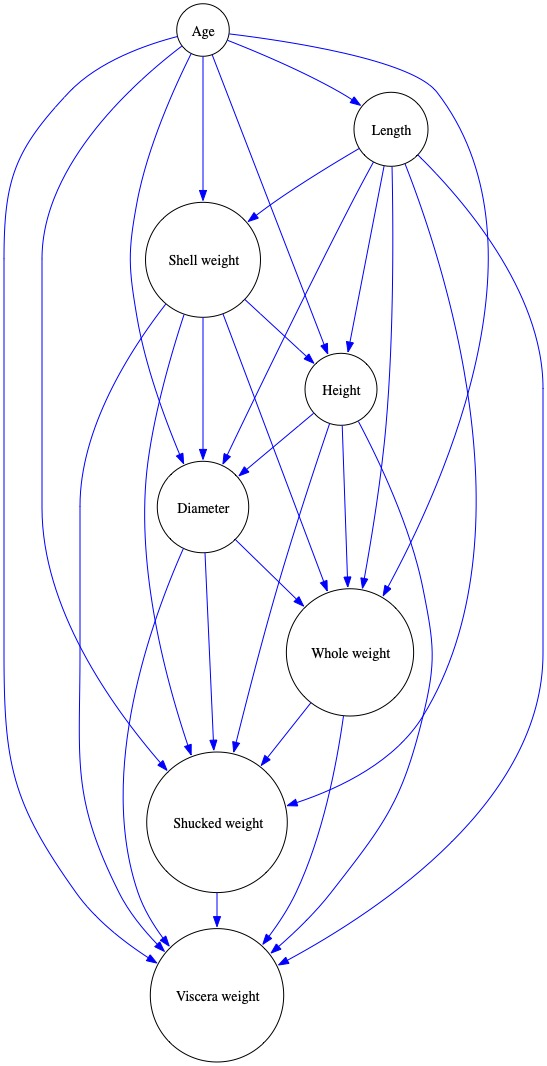
\includegraphics[width=\linewidth]{./demo_data/20241104_093143/Abalone/output_graph/revised_graph.pdf}
        \caption{\label{fig:corr}Revised Graph}
    \end{figure}
\end{minipage}

\subsection{Graph Reliability Analysis}
\begin{figure}[H]
    \centering
    \begin{subfigure}{0.32\textwidth}
        \centering
        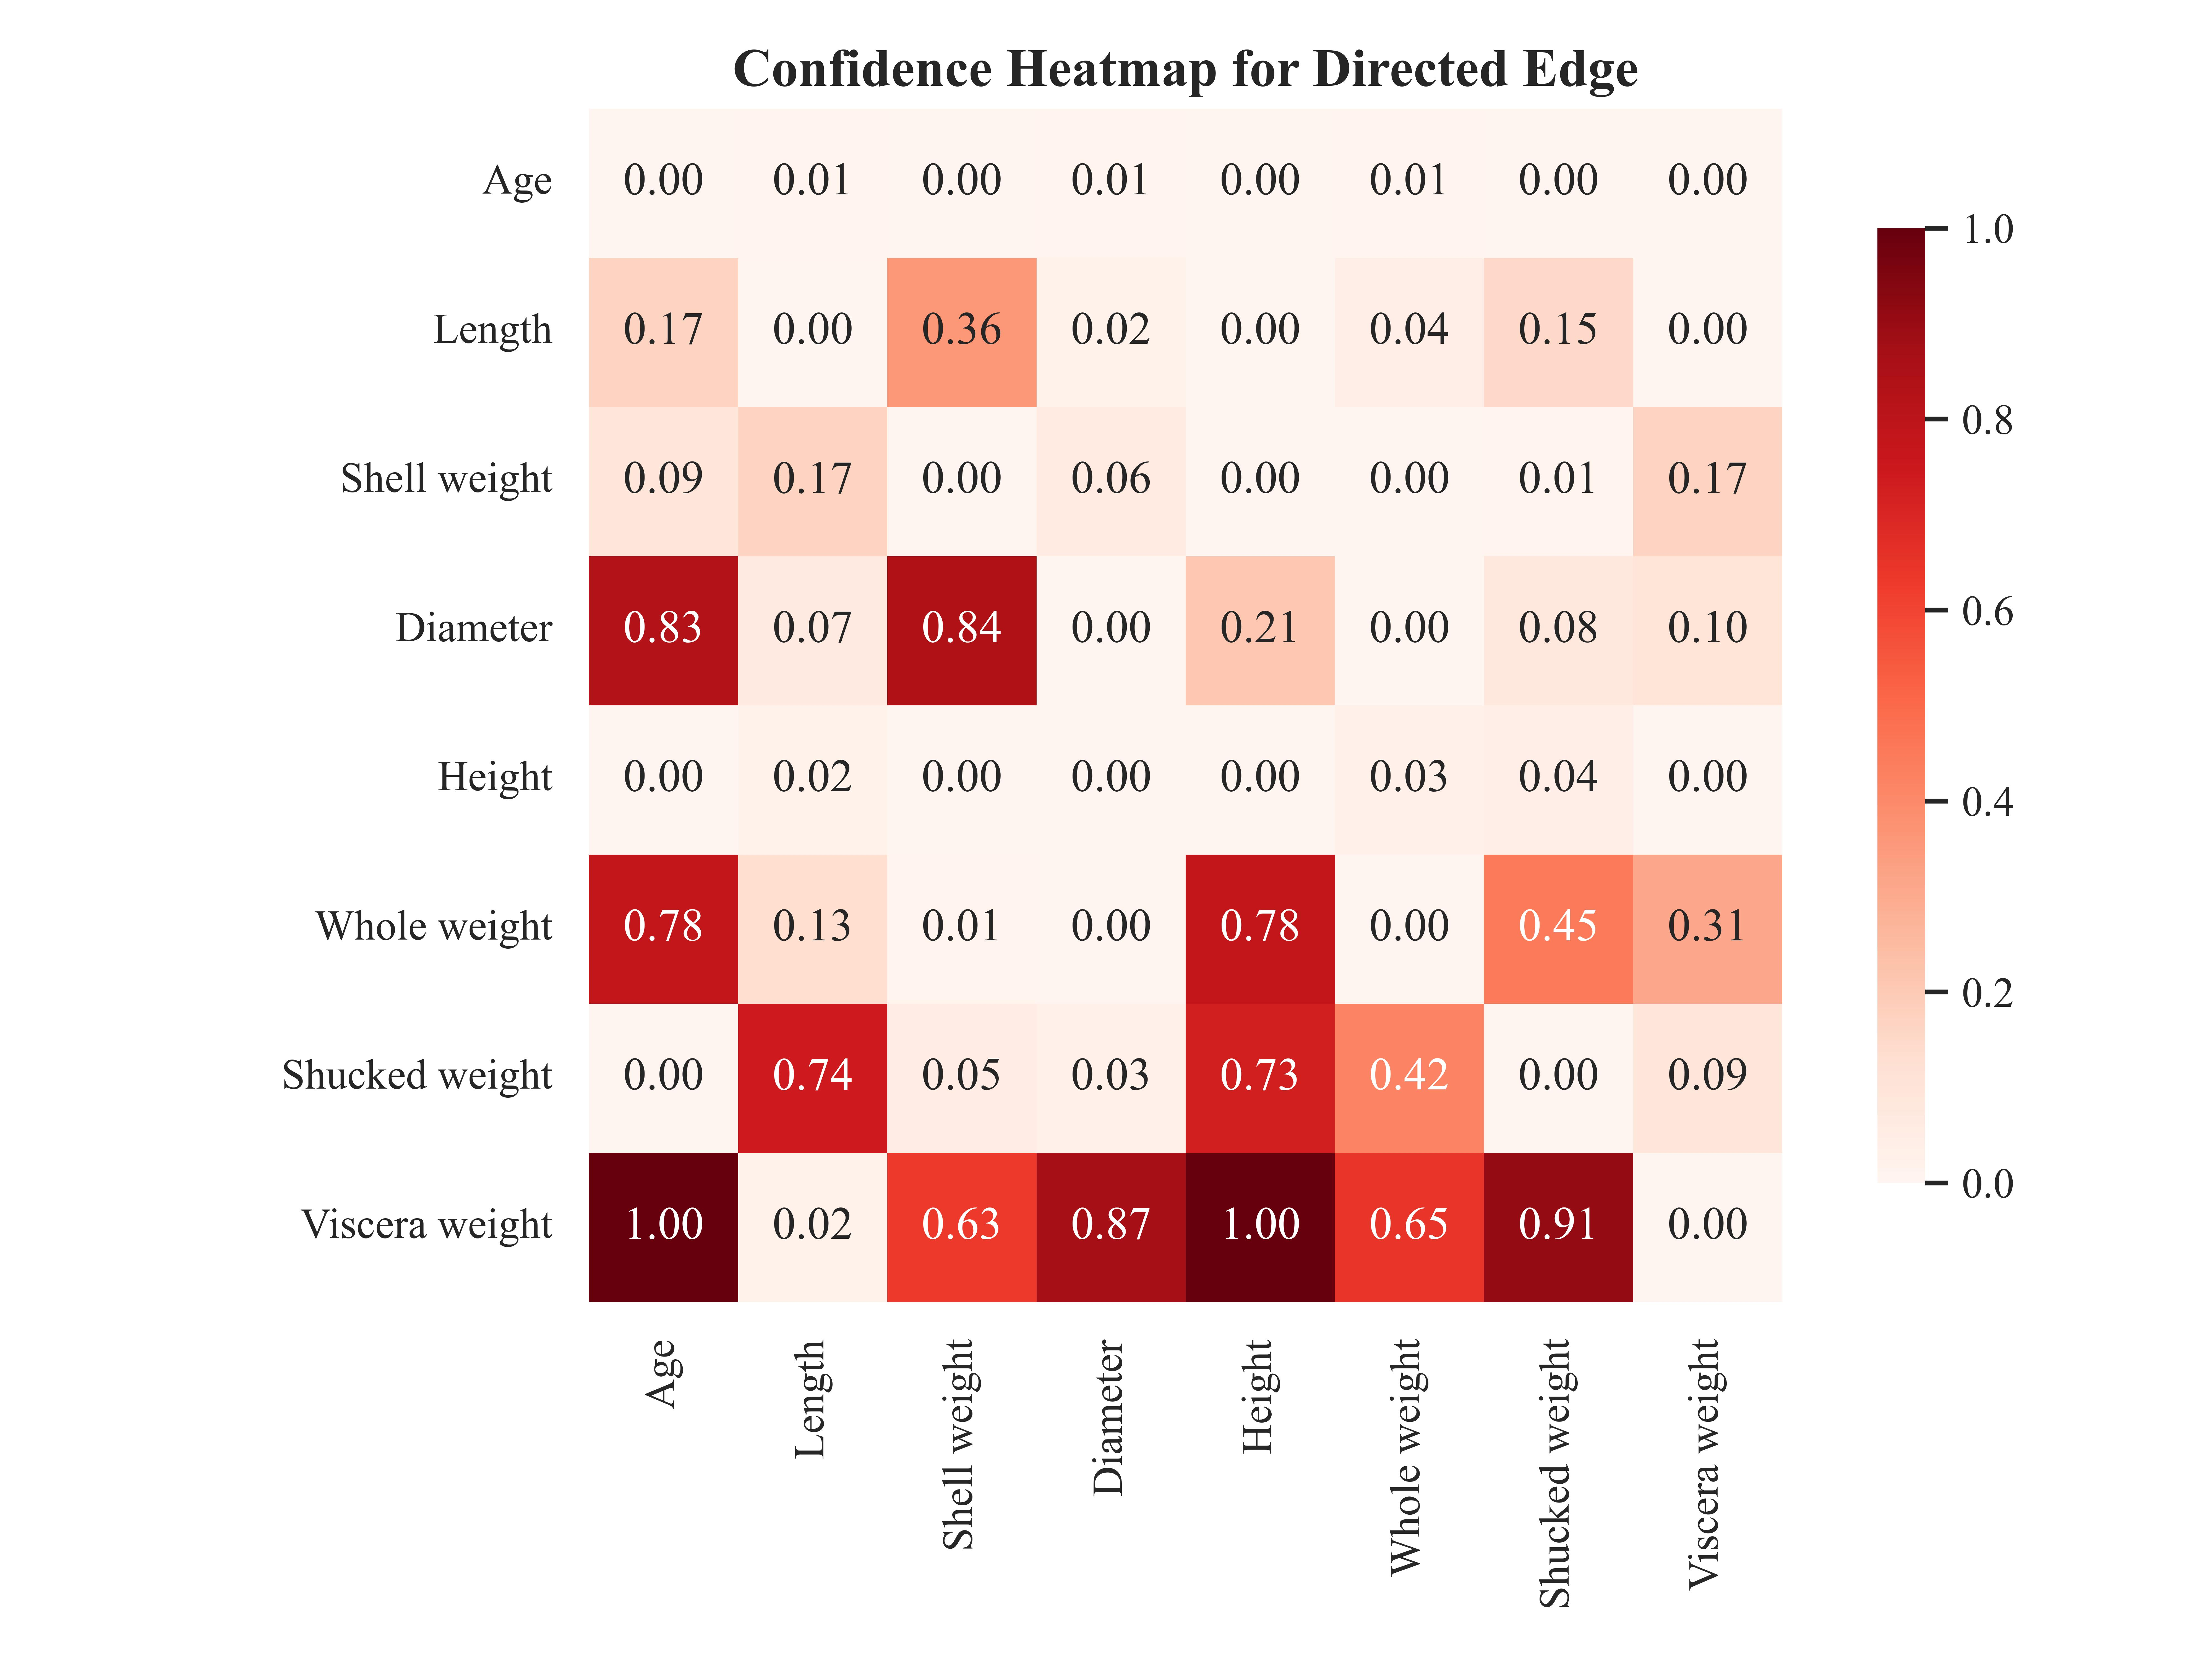
\includegraphics[width=\linewidth]{./demo_data/20241104_093143/Abalone/output_graph/certain_edges_confidence_heatmap.jpg}
        \caption{Directed Edge Edge}
    \end{subfigure}
    \begin{subfigure}{0.32\textwidth}
        \centering
        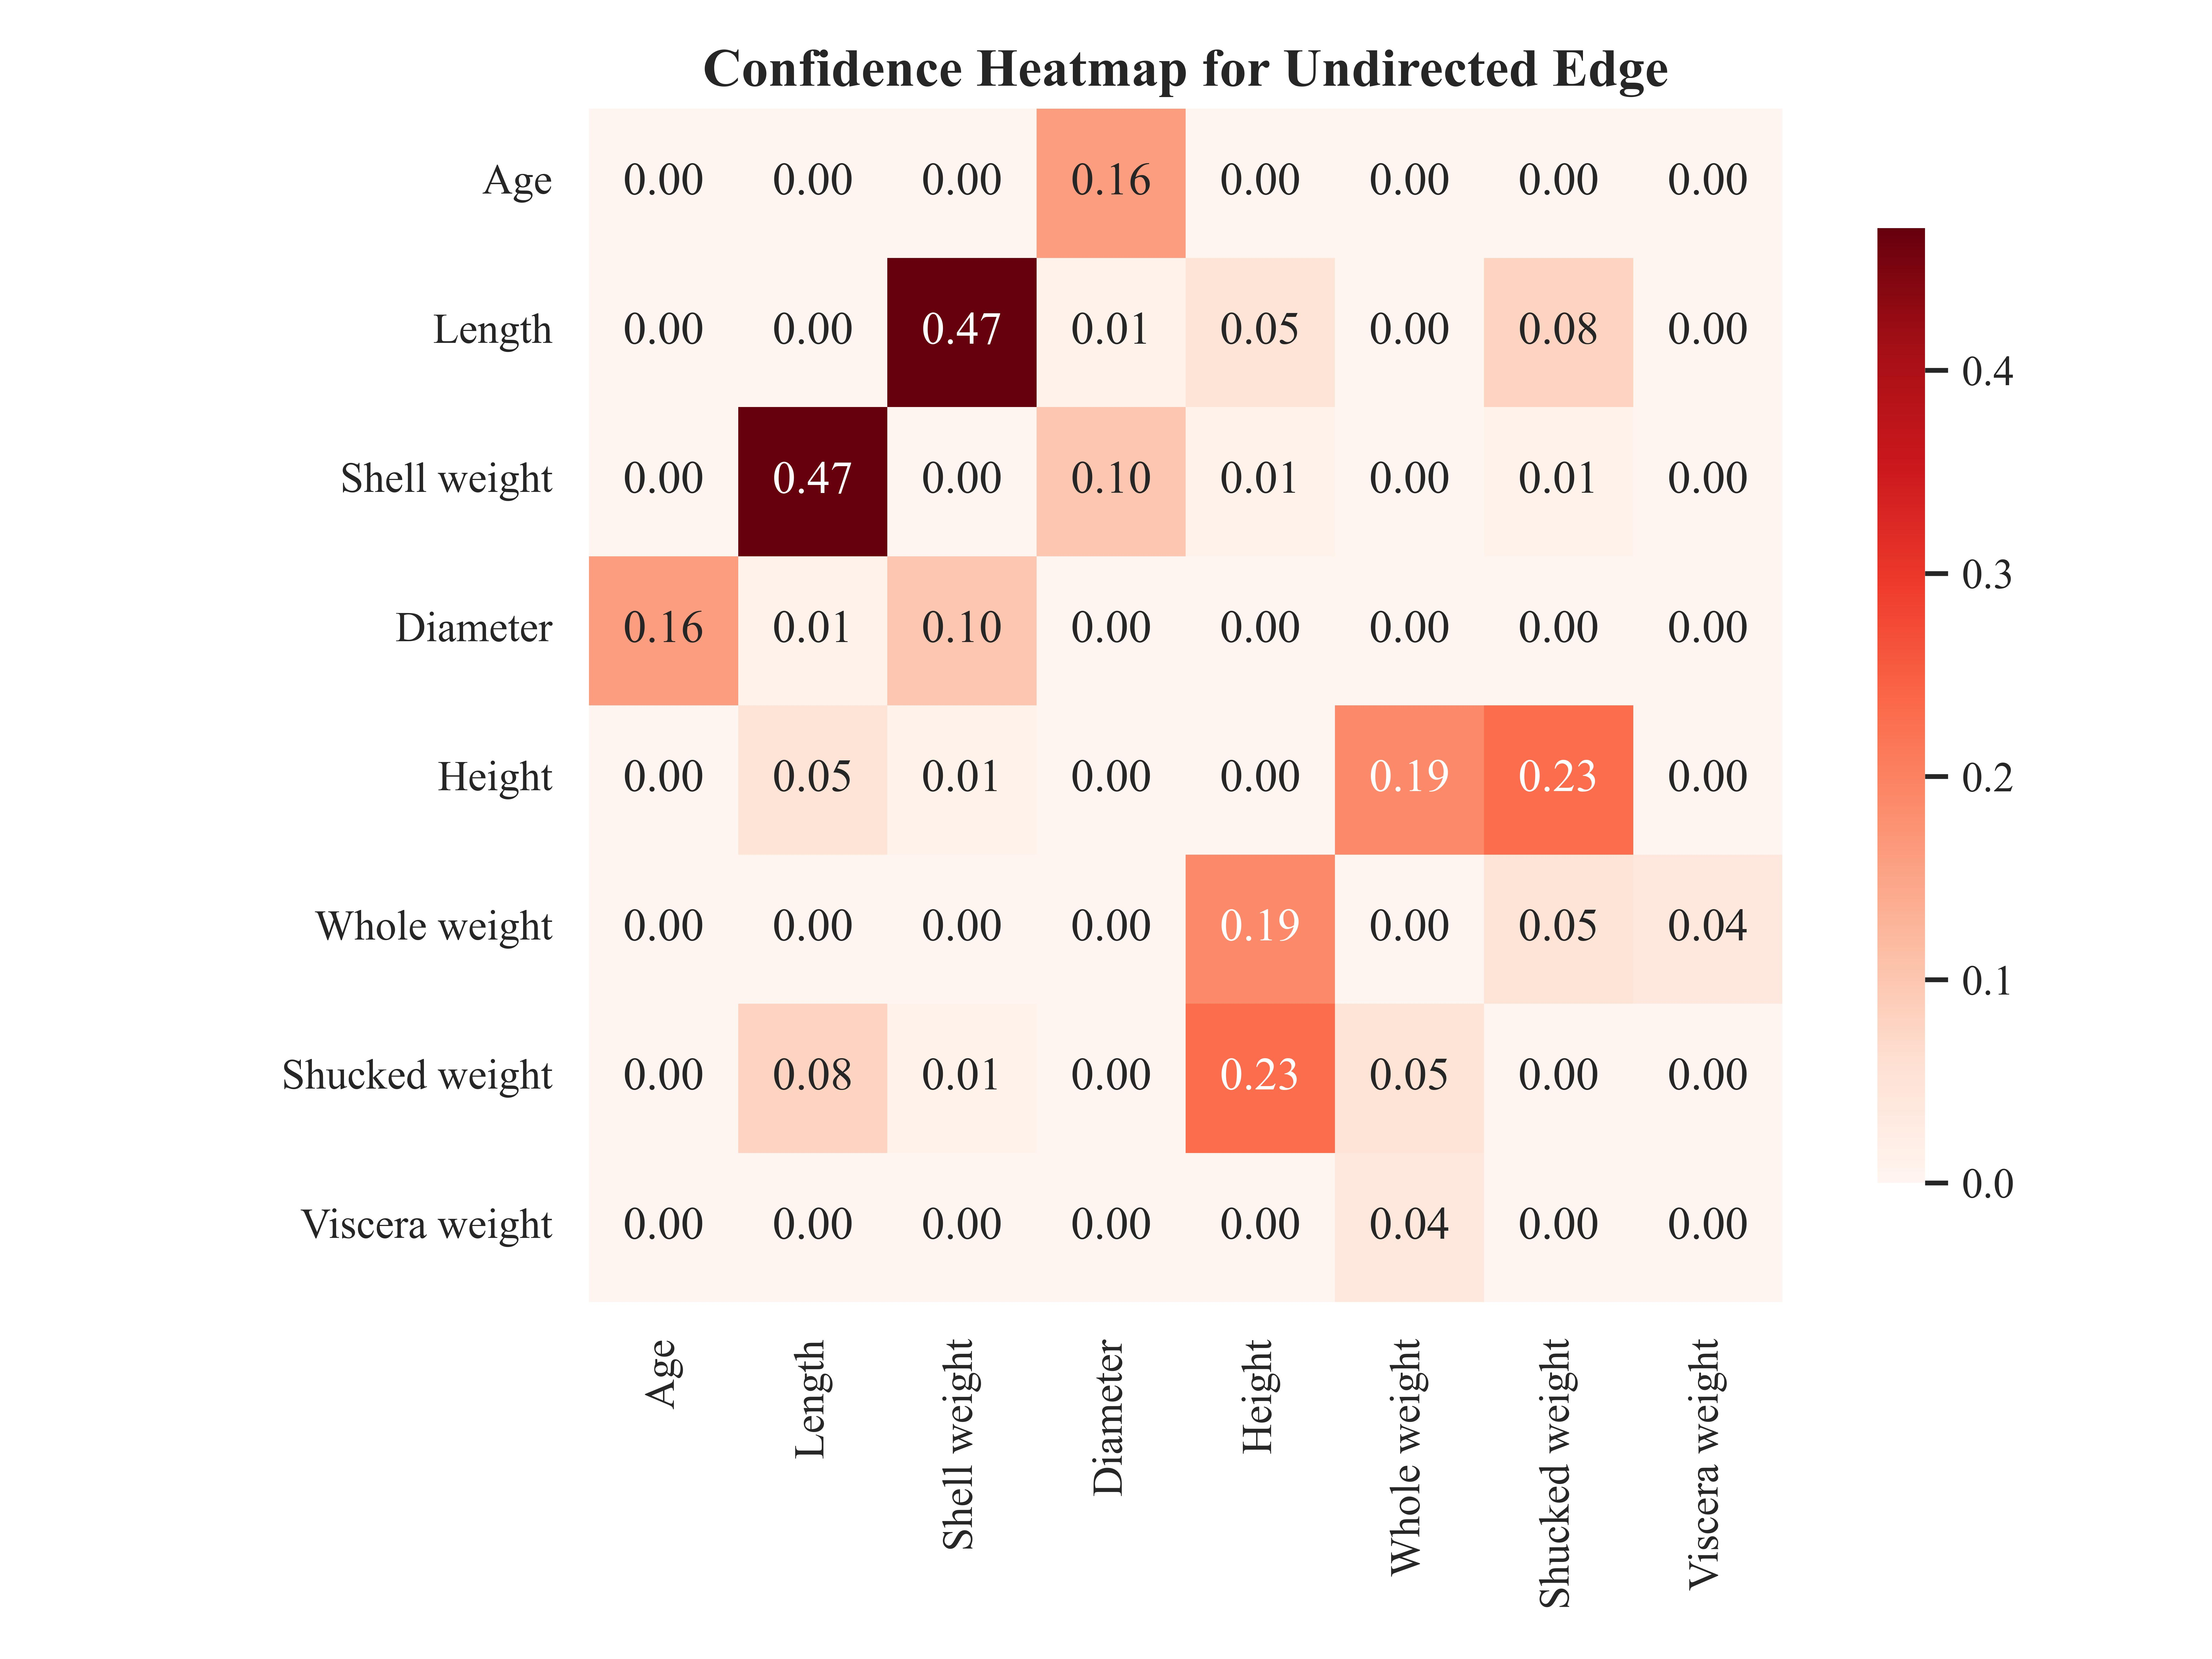
\includegraphics[width=\linewidth]{./demo_data/20241104_093143/Abalone/output_graph/uncertain_edges_confidence_heatmap.jpg}
        \caption{Undirected Edge Edge}
    \end{subfigure}
    \begin{subfigure}{0.32\textwidth}
        \centering
        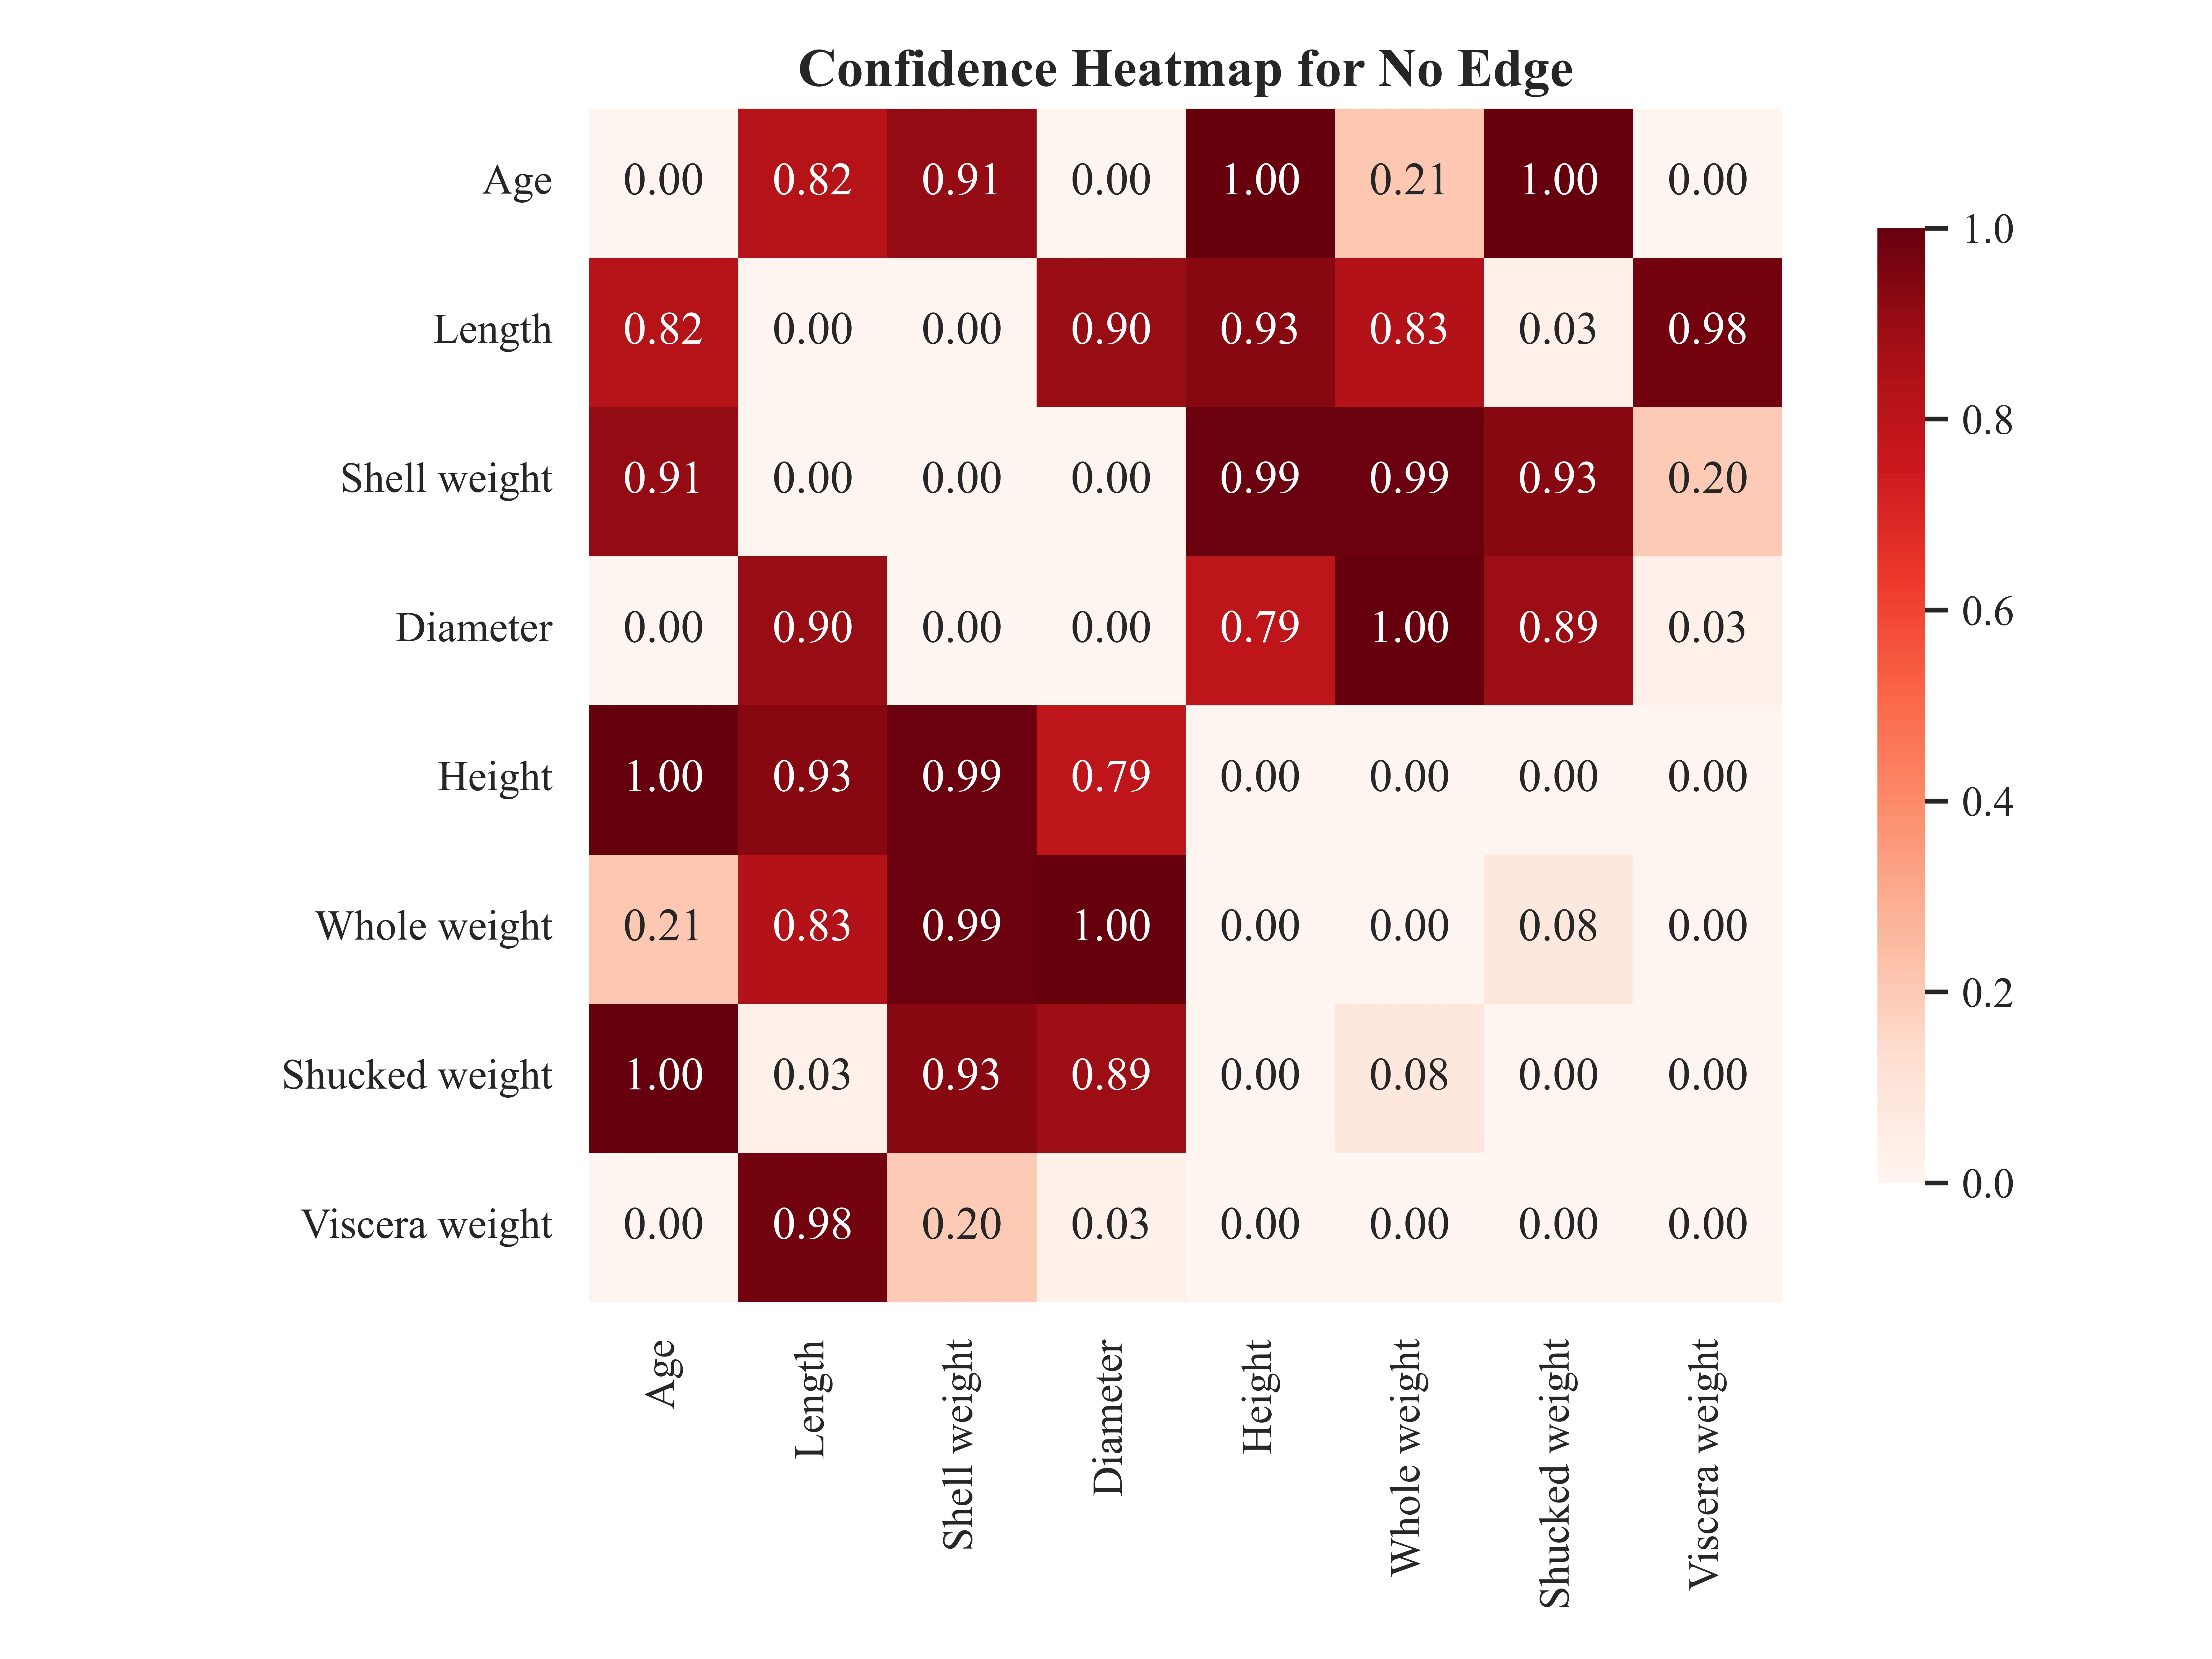
\includegraphics[width=\linewidth]{./demo_data/20241104_093143/Abalone/output_graph/non_existence_confidence_heatmap.jpg}
        \caption{No Edge Edge}
    \end{subfigure}
    \caption{Confidence Heatmap of Different Edges}
\end{figure}        
The above heatmaps show the confidence probability we have on different kinds of edges, including directed edge ($\rightarrow$), undirected edge ($-$), No Edge, and probability of no edge. The heatmap of bi-edges is not shown because probabilities of all edges are 0. Based on the confidence probability heatmap and background knowledge, we can analyze the reliability of our graph.

From the statistics perspective, we have high confidence to believe that the edges with significant bootstrap probabilities exist, particularly the relationships between Whole weight and the other weight measures (Height, Shucked weight, and Viscera weight) with probabilities of 0.78, 0.45, and 0.31, respectively. Additionally, the edge from Age to Length (bootstrap probability of 0.36) is also more plausible, whereas the edges such as Age $\rightarrow$ Diameter (0.01), Age $\rightarrow$ Viscera weight (0.0), and Height $\rightarrow$ Diameter (0.0) suggest a very low confidence in these causal relationships existing. 

However, based on expert knowledge, we know that Age likely influences Length, Height, and overall weight measures, making some of the lower probability edges, despite their statistical values, plausible when contextualized with biological growth patterns in abalones. Notably, we can be reasonably confident that the influence of Length on Shell weight and Shucked weight can exist due to their natural interdependencies. Nonetheless, some edges with very low bootstrap probabilities, like Height $\rightarrow$ Viscera weight (0.0) and Age $\rightarrow$ Viscera weight (0.0), are less grounded in biological reality.

Therefore, the result of this causal graph is partially reliable, but caution should be exercised, particularly around the edges with the lowest confidence. These relationships should be further investigated to refine our understanding of the underlying biology influencing the abalone's growth and characteristics.

\end{document}